\documentclass{beamer}

\mode<presentation>
\usetheme{Madrid}
\definecolor{Columbia}{RGB}{185,217,235}
\definecolor{Columbia2}{RGB}{0,51,160}
\definecolor{Columbia3}{RGB}{0,114,206}
\setbeamercolor{title}{fg=Columbia2}
\setbeamercolor{frametitle}{fg=Columbia2}
\setbeamercolor{block title}{bg=Columbia, fg=Columbia2}
%\setbeamercolor{block body}{fg=Columbia2}
\setbeamercolor{structure}{fg=Columbia}
\setbeamercolor{item projected}{fg=white}
\setbeamercolor{item}{fg=Columbia2}
\setbeamercolor{subitem}{fg=Columbia2}
\setbeamercolor{section in toc}{fg=Columbia}
\setbeamercolor{description item}{fg=Columbia}
\setbeamercolor{caption name}{fg=Columbia}
\usepackage{graphics}
\usepackage{geometry}
\usepackage{booktabs}
\usepackage{multirow, makecell}
\usepackage{float}
\usepackage{fancyvrb}
\usepackage{caption}
\usepackage{subcaption}
\usepackage{adjustbox}
\usepackage{hyperref}

%\hypersetup{
%colorlinks=true,
%linkcolor=black,
%filecolor=green, 
%urlcolor=blue,
%}
\beamertemplatenavigationsymbolsempty
\setbeamertemplate{footline}[page number]
\setbeamercolor{page number in head/foot}{fg=black}
\setbeamertemplate{headline}{}
\makeatletter
\let\@@magyar@captionfix\relax
\makeatother


\title[Econometrics 2]{Introduction to Econometrics 2: Recitation 12} % Change this regularly
\author{Seung-hun Lee}
\institute{Columbia University}

\date{April 29th, 2020}

\begin{document}
\begin{frame}
\titlepage
\end{frame}
%%%%%%%%%%%%%%%

\begin{frame}
\frametitle{Regression Discontinuity}
Introduction 
\begin{itemize}
\item \textbf{Regression discontinuity} was brought into the mainstream of applied economics very recently.
\item Whenever you learn applied microeconomics class in your second year, you are bound to read or present about a paper that uses this research design.
\item This approach exploits the discontinuities in the treatment assignment. 
\begin{itemize} 
\item So the key difference between regression discontinuity and previous frameworks is that RDD does not require the overlap condition in the sense that $p(X_i)\in(0,1)$. 
\item In fact, one of the design has $p(X_i)=1$ for $X_i\geq c$ and $0$ otherwise.
\end{itemize}
\end{itemize}
\end{frame}

\begin{frame}
\frametitle{Regression Discontinuity}
Introduction 
\begin{itemize}
\item  Another thing that RDD should satisfy is that for every other covariates, the distribution should remain continuous even through the discontinuity.
\item This is usually presented visually through graphs - one with the covariate that determines assignment to the treatment, usually called the forcing (running) variable $W_i$ and the treatment status $D_i$, the other with the $W_i$ and all other covariates $X_i$. 
\item If we are in the public finance context and study the effect of a particular welfare program with a means-tested benefit assignment mechanism, we could use the means-tested criteria as our $W_i$.
\item If we are to study the effect of a specific educational program offered to those below a particular test score, that score could be the $W_i$.
\end{itemize}
\end{frame}

\begin{frame}
\frametitle{Regression Discontinuity}
Lee (2007, JOEconometrics)
\begin{itemize}
\item  This paper focuses on the elections won/lost by a very narrow margin. 
\item The running variable is the Democrat vote share $-$ Republican vote share, or a margin of victory/loss.
\item One of the findings is that Democrats who barely win an election are much more likely to run for office and succeed in the next election, compared to Democrats who barely lose. (Carries over to other electoral outcomes)
\end{itemize}
Ost, Pan, Webber (2018, JLE)
\begin{itemize}
\item This paper estimates the return to college using admin data on college enrollment and earnings from Ohio.
\item The running variable here is a GPA
\item Dismissal leads to a short-run increase in earnings and tuition savings wiped out by gains from college graduates 8 years after. They also carry out the test that the result is not driven by manipulation.
\end{itemize}
\end{frame}

\begin{frame}
\frametitle{Regression Discontinuity}
Howell (2017, AER)
\begin{itemize}
\item This paper assess the impact of R\&D subsidies from the government to new ventures.
\item The rank on the application to the R\&D is used as a running variable, 
\item The paper finds that an early-stage award approximately doubles the probability that a firm receives subsequent venture capital  and has large, positive impacts on patenting and revenue. \medskip
\begin{figure}[H]
\centering
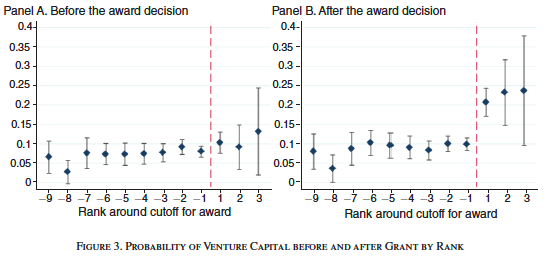
\includegraphics[width=0.6\textwidth, keepaspectratio]{RD_fig.png}
\end{figure}
\end{itemize}
\end{frame}

\begin{frame}
\frametitle{Regression Discontinuity}
Framework
\begin{itemize}
\item We will start with a \textbf{sharp RDD}, where the assignment into the treatment is determined by
\[
D_i=1(W_i\geq c(X_i))
\]
where $c(X_i)$ can be a known function of $X_i$ or just a constant. 
\item We also keep the potential outcome framework from before, but we will slightly change this to
\small{\begin{align*}
Y_i& = D_iY_i(1)+(1-D_i)Y_i(0)\\
&=Y_i(0)+D_i(Y_i(1)-Y_i(0))\\
&=Y_i(0)+1(W_i\geq c(X_i))\cdot(Y_i(1)-Y_i(0))
\end{align*}}\normalsize
\item We also keep the regressional framework for the potential outcomes, $Y_i(d)=\mu(X_i,W_i,d)+\epsilon_i(d)$. So we have
\small{\[
E[Y_i(d)|X_i,W_i]=\mu(X_i.W_i.d)
\]}\normalsize
\end{itemize}
\end{frame}

\begin{frame}
\frametitle{Regression Discontinuity}
Framework
\begin{itemize}
\item One assumption that we carry in this section is the continuity of the conditional expectation on potential outcomes at $W_i=c(X_i)$
\begin{block}{Continuity of $\mu(X_i,W_i,d)$ at $W_i=c$}
If $W_i$ has a known cutoff at $c$, we assume that $E[Y_i(1)|X_i, W_i]$ and $E[Y_i(0)|X_i, W_i]$ are continuous around $W_i=c$. Put if differently, 
\[
E[Y_i(d)|X_i, W_i=c^+]=E[Y_i(d)|X_i, W_i=c^-] \ \text{for each } d\in\{0,1\}
\]
\end{block}
\item The above condition also implies that $(\epsilon_i(1), \epsilon_i(0))$ also has a continuous distribution around $W_i=c(X_i)$.
\item If this condition is not satisfied, this implies that there could be more than the $W_i$ variable that jumps around the cutoff
\end{itemize}
\end{frame}

\begin{frame}
\frametitle{Regression Discontinuity}
Fuzzy RDD Framework
\begin{itemize}
\item There is another version of the RDD which is more general than the sharp RDD.
\item A \textbf{fuzzy RDD} setup exploits the jump in the probability of being treated at $W_i=c$. 
\item This jump is not necessarily from 0 to 1. 
\item Formally, we say we look for discontinuities of 
\[
\Pr(D_i|X_i,W_i)
\]
at $W_i=c(X_i)$. 
\end{itemize}
\end{frame}

\begin{frame}
\frametitle{Regression Discontinuity}
Identification: Sharp RDD
\begin{itemize}
\item  Assume that $c(X_i)$ is a constant $c$. We can write
\footnotesize{\begin{align*}
E[Y_i|X_i, W_i]&=E[Y_i(0)|X_i, W_i]+E[(Y_i(1)-Y_i(0))1(W_i\geq c(X_i))|X_i, W_i]
\end{align*}}\normalsize
\item And we can separate the above into two. One with $W_i=c^+$ and the other with $W_i=c^-$.
\footnotesize{\begin{align*}
E[Y_i|X_i, W_i=c^+]&=E[Y_i(0)|X_i, W_i=c^+]+E[(Y_i(1)-Y_i(0))|X_i, W_i=c^+]\\
E[Y_i|X_i, W_i=c^-]&=E[Y_i(0)|X_i, W_i=c^-]
\end{align*}}\normalsize
\item  Therefore, 
\footnotesize{\begin{align*}
E[Y_i|X_i, W_i=c^+] - E[Y_i|X_i, W_i=c^-]&=E[Y_i(0)|X_i, c^+]-E[Y_i(0)|X_i, c^-]\\ &+E[(Y_i(1)-Y_i(0))|X_i, c^+]
\\&=E[(Y_i(1)-Y_i(0))|X_i, c^+]
\end{align*}}\normalsize
where the first line on the right hand side vanishes due to the continuity assumptions.
\end{itemize}
\end{frame}

\begin{frame}
\frametitle{Regression Discontinuity}
Identification: Sharp RDD
\begin{itemize}
\item Reusing the continuity argument, we can write  
\[
E[(Y_i(1)-Y_i(0))|X_i, W_i=c^+]=E[(Y_i(1)-Y_i(0))|X_i, W_i=c]
\]
\item Therefore, we have backed out
\[
E[(Y_i(1)-Y_i(0))|X_i, W_i=c]=E[Y_i|X_i, W_i=c^+] - E[Y_i|X_i, W_i=c^-]
\]
which is the average treatment effect at $W_i=c$ and a given $X_i$
\item  This is similar to the LATE in the sense if we let $Z_i=1(W_i\geq c)$, we can get back what is effectively equivalent to the LATE estimator (with the difference in the probability of treatment exactly at 1).
\item Also, we are looking at the treatment effect on the compliers, albeit a very narrow group of people.
\end{itemize}
\end{frame}

\begin{frame}
\frametitle{Regression Discontinuity}
Identification: Fuzzy RDD
\begin{itemize}
\item For the fuzzy RDD, we can write as follows 
\footnotesize{\begin{align*}
E[Y_i|X_i, W_i]&=E[Y_i(0)|X_i, W_i]+E[(Y_i(1)-Y_i(0))\Pr(D_i=1|X_i, W_i)|X_i, W_i]
\end{align*}}\normalsize
So we can do the similar approach as in sharp RDD and get 
\footnotesize{\begin{align*}
E[Y_i|x, c^+]&=E[Y_i(0)|x, c^+]+\Pr(D_i=1|x,c^+)E[Y_i(1)-Y_i(0)|x, c^+]\\
E[Y_i|x, c^-]&=E[Y_i(0)|x, c^-]+\Pr(D_i=1|x, c^-)E[Y_i(1)-Y_i(0)|x, c^-]
\end{align*}}\normalsize
\item So using the continuity assumption, the difference in the LHS is
\footnotesize{\[
E[Y_i|x, c^+]-E[Y_i|x, c^-]=[\Pr(D_i=1|x, c^+)-\Pr(D_i=1|x, c^-)]E[Y_i(1)-Y_i(0)|x, c]
\]}\normalsize
\item Thus, we also identify an average treatment effect at $W_i=c$ and $X_i=x$, which is now divided by something that is not necessarily 1. 
\footnotesize{\[
E[Y_i(1)-Y_i(0)|X_i, W_i=c]=\frac{E[Y_i|X_i, W_i=c^+]-E[Y_i|X_i, W_i=c^-]}{\Pr(D_i=1|x, W_i=c^+)-\Pr(D_i=1|x, W_i=c^-)}
\]}\normalsize
\end{itemize}
\end{frame}

\begin{frame}
\frametitle{Regression Discontinuity}
Implementation: Nonparametrics
\begin{itemize}
\item One way to implement RDD in practice is to make use of nonparametric regression. 
\item The bandwidth, however, should be bounded at $c$.
\begin{itemize}
\item If you are doing a nonparametric regression from the left of the bandwidth, you should apply this on $[c-\epsilon, c)$
\item For the right hand side, $[c, c+\epsilon]$. 
\item If the domain reaches beyond $c$ from either side, there is a huge risk of misfitting the data.
\end{itemize}
\item Ideally, carry out a local linear (or polynomial) regression
\item We also run into curse of dimensionality and minimizing AMISE in determining optimal bandwidth (bias-variance tradeoff).
\item Calonico, Cattaneo, and Tituinik (2014) suggests the use of local quadratic estimator with the optimal bandwidth selected by the minimization of AMISE, which is typically known as IK bandwidth (Imbens, Kalyanaraman, 2012).
\end{itemize}
\end{frame}

\begin{frame}
\frametitle{Regression Discontinuity}
Implementation: Parametrics
\begin{itemize}
\item One way is to run a separate regression for both left and right of the cutoff. That is, run
\footnotesize{\begin{gather*}
Y_i = X_i\beta^- +(c-w_i)X_i\gamma^-+\epsilon_i^-\ \ \text{for }w_i<c\\
Y_i = X_i\beta^+ +(w_i-c)X_i\gamma^++\epsilon_i^+\ \ \text{for }w_i\geq c
\end{gather*}}\normalsize
allowing us to fit a different trend on the left \& right of the cutoff $c$. 
\item There is also a way in which we make use of both sides of the cutoff. Specifically, we run
\[
Y_i = X_i\beta+ X_i \cdot 1(W_i\geq c)\gamma+X_i\cdot(c-W_i)\delta+X_i\cdot (c-W_i)\cdot 1(W_i\geq c) \mu +\epsilon_i
\]
Here, what happens is that
\begin{itemize}
\item $W_i\geq c$: $Y_i=X_i(\beta+\gamma)+X_i\cdot(c-W_i)(\delta+\mu)$
\item $W_i< c$: $Y_i=X_i(\beta)+X_i\cdot(c-W_i)(\delta)$
\end{itemize}
\item In an $(Y_i, W_i)$ plane, $\gamma$ captures the jump, $\delta, \mu$ determines slope
\end{itemize}
\end{frame}

\begin{frame}
\frametitle{Regression Discontinuity}
Implementation: Diagnostics
\begin{itemize}
\item First, we plot $Y_i$ as a function of $W_i$ for a given $X_i$ and see if there is a mean shift. 
\item We plot the propensity score $\Pr(D_i=1|X_i, W_i)$ and look for a shift.
\item One thing that should not shift is the distribution of $X_i$'s. So plot $X_i$'s as function of $W_i$ and confirm that there is no shift. 
\item Another thing to worry regarding $W_i$ is the possibility of manipulating or gaming. Therefore, use a McCrary test to confirm that the distribution of $W_i$ do not change at $W_i=c$.  (No bunching!)
\item What if we do not know the exact cutoff? We can figure out what they might be based on the distribution of $W_i$ (Chay, McEwan, and Urquiola, 2005)
\item We lose a lot of data in selecting the optimal bandwidth around the cutoff, hurting external validity.
\end{itemize}
\end{frame}

\begin{frame}
\frametitle{Machine Learning}
Introduction
\begin{itemize}
\item Machine learning in the context of econometrics is interested in model selection for prediction - finding the parsimonious model in the context of a very large dataset. 
\item It ranges from regularized models such as LASSO, Ridge regression, and elastic nets and methods that are much more involved - random forests and neural networks. 
\item Often, we are interested in controlling a large set of covariates 
\item In determining the structure, we face a trade-off: We are tempted to increase the number of covariates to fit the data better. 
\item However, in doing so, we risk overfitting - the out-sample prediction can perform poorly in terms of variance.
\item Therefore, some method to penalize complexity is required. 
\end{itemize}
\end{frame}

\begin{frame}
\frametitle{Machine Learning}
Information Criterion
\begin{itemize}
\item We start with a set $\mathcal{M}$ of candidate models. Then for $M\in\mathcal{M}$, we define a penalty parameter $p(M)$ that increases in complexity. 
\begin{itemize}
\item Akaike's Information Criterion: Choose $M$ satisfying
\[
\max_{M}\left(\max_\theta \sum_{i=1}^n \log{l_i(\theta;M)}-p(M) \right)
\]
\item Bayesian Information Criterion: Choose $M$ satisfying
\[
\max_{M}\left(\max_\theta \sum_{i=1}^n \log{l_i(\theta;M)}-p(M)\frac{\log{n}}{2} \right)
\]
\end{itemize}
\item  BIC tends to be harsher for complexities and performs better for model selection
\item For out-sample performance, AIC performs better. 
\item Both of them, however, can be impractical to calculate when we work with large models. If $p$ is a number of potential covariates, and $n$ is the sample size, we run into the case where $p>>n$. 
\end{itemize}
\end{frame}

\begin{frame}
\frametitle{Machine Learning}
Shrinkage
\begin{itemize}
\item One way out is to penalize complexities with the convex norm penalties. Define
\[
\Vert \theta \Vert _m = \sqrt[m]{\sum_{k=1}^p \vert \theta_k \vert ^m}
\]
and for $m=0$, we have $\Vert \theta \Vert _p=p$
\item Depending on the selection of $m$, we get different estimators that incorporates different shrinkage mechanisms 
\item The general idea of shrinkage is as follows: We know that OLS is BLUE. But what if we are willing to relax the 'unbiased' condition? Then can we find some estimators that have lower variance and even a lower mean squared error? James, Stein (1961) shows that it is possible and generalizable.
\end{itemize}
\end{frame}

\begin{frame}
\frametitle{Machine Learning}
LASSO and Ridge
\begin{itemize}
\item Ridge regression minimizes
\[
\sum_{i=1}^n(Y_i-X_i\theta_0)^2+\lambda\sum_{k=1}^p \theta_k^2 
\]
and yields
\[
\hat{\theta} = (X'X+\lambda I_p)^{-1}X'y
\]
\item With LASSO, the minimization is 
\[
\frac{1}{n}\sum_{i=1}^n(Y_i-X_i\theta_0)^2+\lambda\sum_{k=1}^p |\theta_k| 
\]
and the first order condition can be written as
\[
\frac{2}{n}\sum_i X_{ik}(y_i-X_i\theta)=\lambda s_k,
\]
Where $\lambda s_k$ is not necessarily 0, consistent with the idea that we allow for some bias in order to find an estimator that reduces MSE. 
\end{itemize}
\end{frame}

\begin{frame}
\frametitle{Machine Learning}
So what is the difference between LASSO and Ridge? 
\begin{itemize}
\item Ridge regression drives your coefficients towards 0 but not equal to it.
\item So when it comes to model selection in terms of ruling out irrelevant variables, LASSO does better. 
\item Ridge has quicker computation and works better with multicollinearity.  
\item So the choice of the estimation method depends on your goal of minimizing MSE as well as computation power
\begin{figure}[H]
\centering
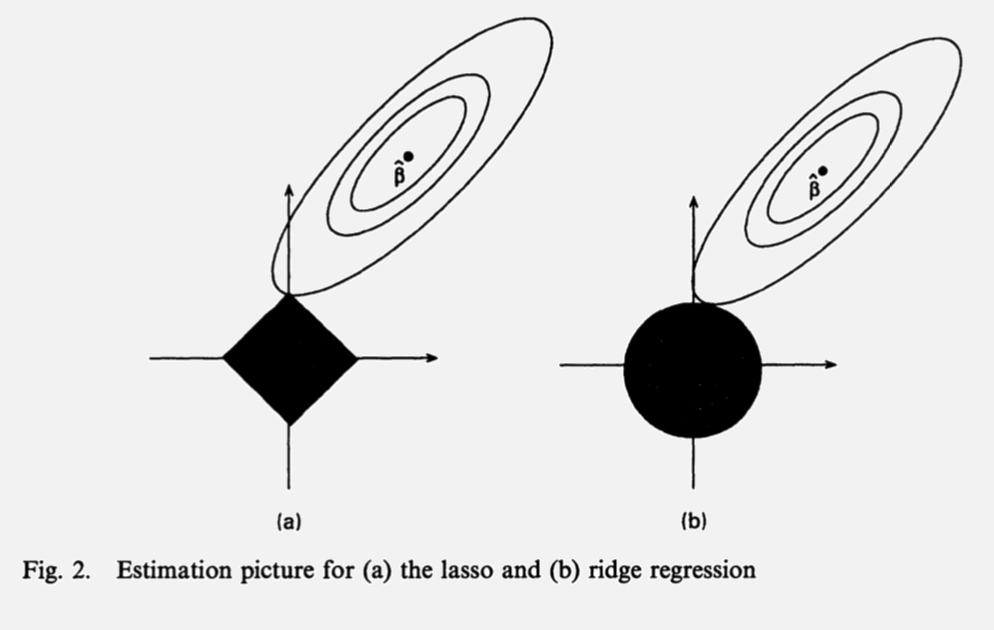
\includegraphics[width=0.5\textwidth, keepaspectratio]{lasso.png}
\end{figure}
\end{itemize}
\end{frame}

\begin{frame}
\frametitle{Machine Learning}
Elastic Net abd LARS
\begin{itemize}
\item The idea of \textbf{elastic net} is to use a penalty term that is a convex combination of both $l_1$ and $l_2$ penalty term. Specifically, 
\[
\sum_{i=1}^n(Y_i-X_i\theta_0)^2+\lambda\sum_{k=1}^n\left[\alpha \Vert \theta \Vert_1^2 +(1-\alpha)\Vert \theta \Vert_2^2\right]
\]
\item If $\lambda=0$ we have an OLS. For $\lambda\neq0$, if $\alpha=1$, we have LASSO, and if $\alpha=0$ we get Ridge. 
\end{itemize}
\end{frame}

\begin{frame}
\frametitle{Machine Learning}
Elastic Net abd LARS
\begin{itemize}
\item For \textbf{Least Angle Regression (LARS)} the algorithm is 
\begin{enumerate}
\item Start with a constant model: For all non-constant covariates, coefficients are 0 and $\lambda=\infty$. 
\item Find the covariate that has the largest covariance with the residual. 
\item Change the coefficient for that variable in the same direction as its covariance with the residual until you find a different covariate that has as much covariance.  $\lambda$ decrease and $\theta$ is updated along the way.
\item Change the coefficient for the two variables until you find a third variable with the same covariance with the residual. 
\item Stop when all predictors are in the model
\end{enumerate}
\end{itemize}
\begin{figure}[H]
\centering
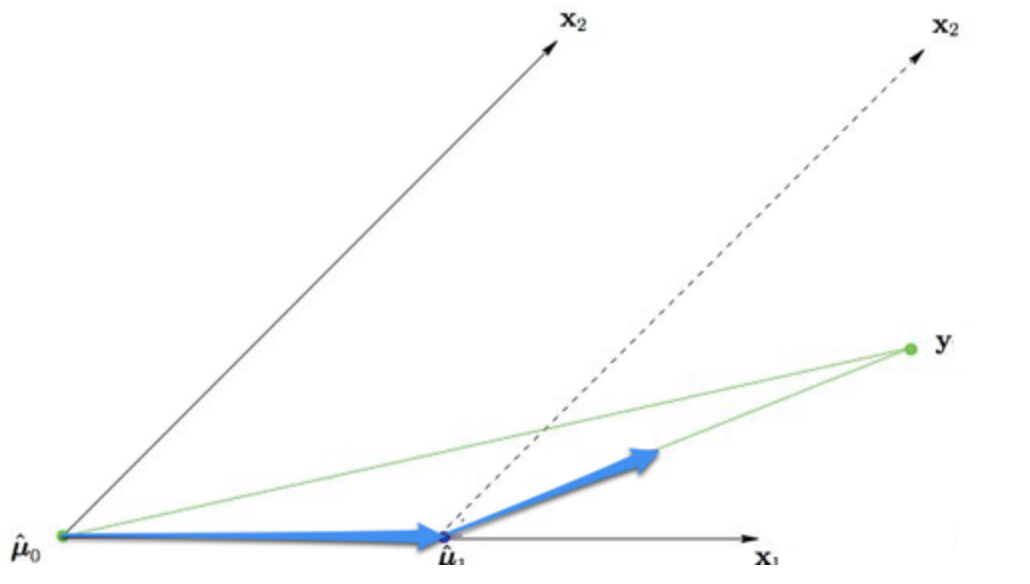
\includegraphics[width=0.4\textwidth, keepaspectratio]{lars.png}
\end{figure}
\end{frame}

\begin{frame}
\frametitle{Machine Learning}
Choosing $\lambda$
\begin{itemize}
\item  If your goal is to minimize the prediction error, you can use the following cross-validation methods to come up with one
\begin{itemize}
\item Leave-one-out: Leave one observation out at a time
\item Training vs Test sample: You split the sample into two, build a model given some $\lambda$ and gain prediction error from the test sample. Then, select $\lambda$ minimizing the prediction error there.
\item $K$-fold cross validation:  For $K-1$ blocks, estimate the model given some $\lambda$ and compute the error on the remaining block. Get this for $K$ blocks and compute the average error. Select $\lambda$ minimizing the error. 
\end{itemize}
\item In general, selecting $\lambda$ depends on your goals
\end{itemize}
\end{frame}

\begin{frame}
\frametitle{Machine Learning}
Consistency of LASSO
\begin{itemize}
\item We want to identify what the true model is in a setting with potentially an infinite number of covariates. 
\item To do that, we first set a sparsity assumption, where the number of nonzero coefficients is not too large.
\item As a thought experiment, we increase the number of regressors as $n\to\infty$ in order to approximate the true model.
\item To satisfy the assumption, we require that the number of nonzero regressors to rise at a slower rate than $n$.
\item Specifically, $s_n = o\left(\sqrt{\frac{n}{\log p}}\right)$.
\end{itemize}
\end{frame}

\begin{frame}
\frametitle{Machine Learning}
Consistency of LASSO
\begin{itemize}
\item If we let $\lambda_n = O\left(\sqrt{\frac{\log p}{n}}\right)$ and have $s_n=o\left(\sqrt{\frac{n}{\log p}}\right)$, then we can show that the prediction error goes to 0 and the LASSO estimator is consistent. Or
\[
\frac{1}{n}\sum_i(X_i\hat{\theta}_n-X_i\hat{\theta}_{0n})^2=O_p(\lambda_n^2s_n)
\]
and 
\[
\Vert \hat{\theta}_n-\hat{\theta}_{0n}\Vert_1 = o_p(\lambda_n s_n) = o_p(1)
\]
\item This comes at the cost of a slightly slower rate of convergence, which is tolerable as long as it is faster than $n^{-1/4}$
\end{itemize}
\end{frame}
%%%%%%%%%%%
\end{document}
